\begin{flushleft}
	\textsl{It is a fact of sociology that topologists}\\
	\textsl{are interested in quadratic forms.}\\
	\rule[0pt]{17em}{0.5pt}\\
	\textsl{-- Serge Lang}
	\vspace{2em}
\end{flushleft}

The goal of this chapter is to construct 

\begin{convention*}
	In this chapter, $\H$ denotes singular (co)homology.
\end{convention*}

\begin{theorem}\label{thm:signature_8_existence_theorem}
	For any $t\in \Z$, there is a framed $4k$-manifold $M$ bounding a homotopy sphere and with signature $\sigma(M)=8t$.
\end{theorem}

\begin{theorem}
\end{theorem}

\section{Quadratic Forms}

For this section, 
Let $M_n(R)$ be the ring of $n\times n$ matrices taking values in $R$. A matrix $Q\in M_n(R)$ is invertible if it's determinant $\det Q\in R$ is a unit, and we denote the group of invertible $n\times n$ matrices by $\GL_n(R)$. Two matrices $Q$ and $P$ are said to be conjugate if $P = \Lambda^\intercal Q\Lambda$ for some invertible matrix $\Lambda\in \GL_n(R)$. Given a matrix $Q$ acting on a free $R$-module $R^n$, there is a bilinear form defined by
\[
	Q(v,w) = v^\intercal Q w\quad \textrm{for all }v,w\in R^n.
\]
We abuse notation by referring to the matrix and the form interchangeably.
Note that the bilinear form only depends on the matrix conjugacy class, and the form is independent of the basis for $R^n$.
Similarly, if we have a bilinear form $Q$, we can define the matrix $Q$ in some basis $\{e_1,\ldots, e_n\}\subset R^n$ by setting $Q_{ij}= Q(e_i, e_j)$. 

Let $\Sym_n(R)$ be the subring of symmetric matrices. There is a bijective correspondence
\[
	\Sym_n(R) / \textrm{conjugation} \quad\iff\quad 
\]

\begin{definition}
\end{definition}

\begin{theorem}\label{thm:signature_divisible_by_8}
	Let $M$ be a highly-connected framed $4k$-manifold whose boundary is either empty or a homotopy sphere. Then the signature $\sigma(M)$ is divisible by $8$.
\end{theorem}

\[
	\begin{pmatrix}
		2 & 1 &   &   &   &   &   &   \\
		1 & 2 & 1 &   &   &   &   &   \\
		  & 1 & 2 & 1 &   &   &   &   \\
		  &   & 1 & 2 & 1 &   &   &   \\
		  &   &   & 1 & 2 & 1 & 0 & 1 \\
		  &   &   &   & 1 & 2 & 1 & 0 \\
		  &   &   &   & 0 & 1 & 2 & 0 \\
		  &   &   &   & 1 & 0 & 0 & 2 \\
	\end{pmatrix}
\]

\section{Plumbing Disk Bundles}

Let $X$ be an $n$-dimensional bundle.


\begin{figure}[ht]
	\centering
	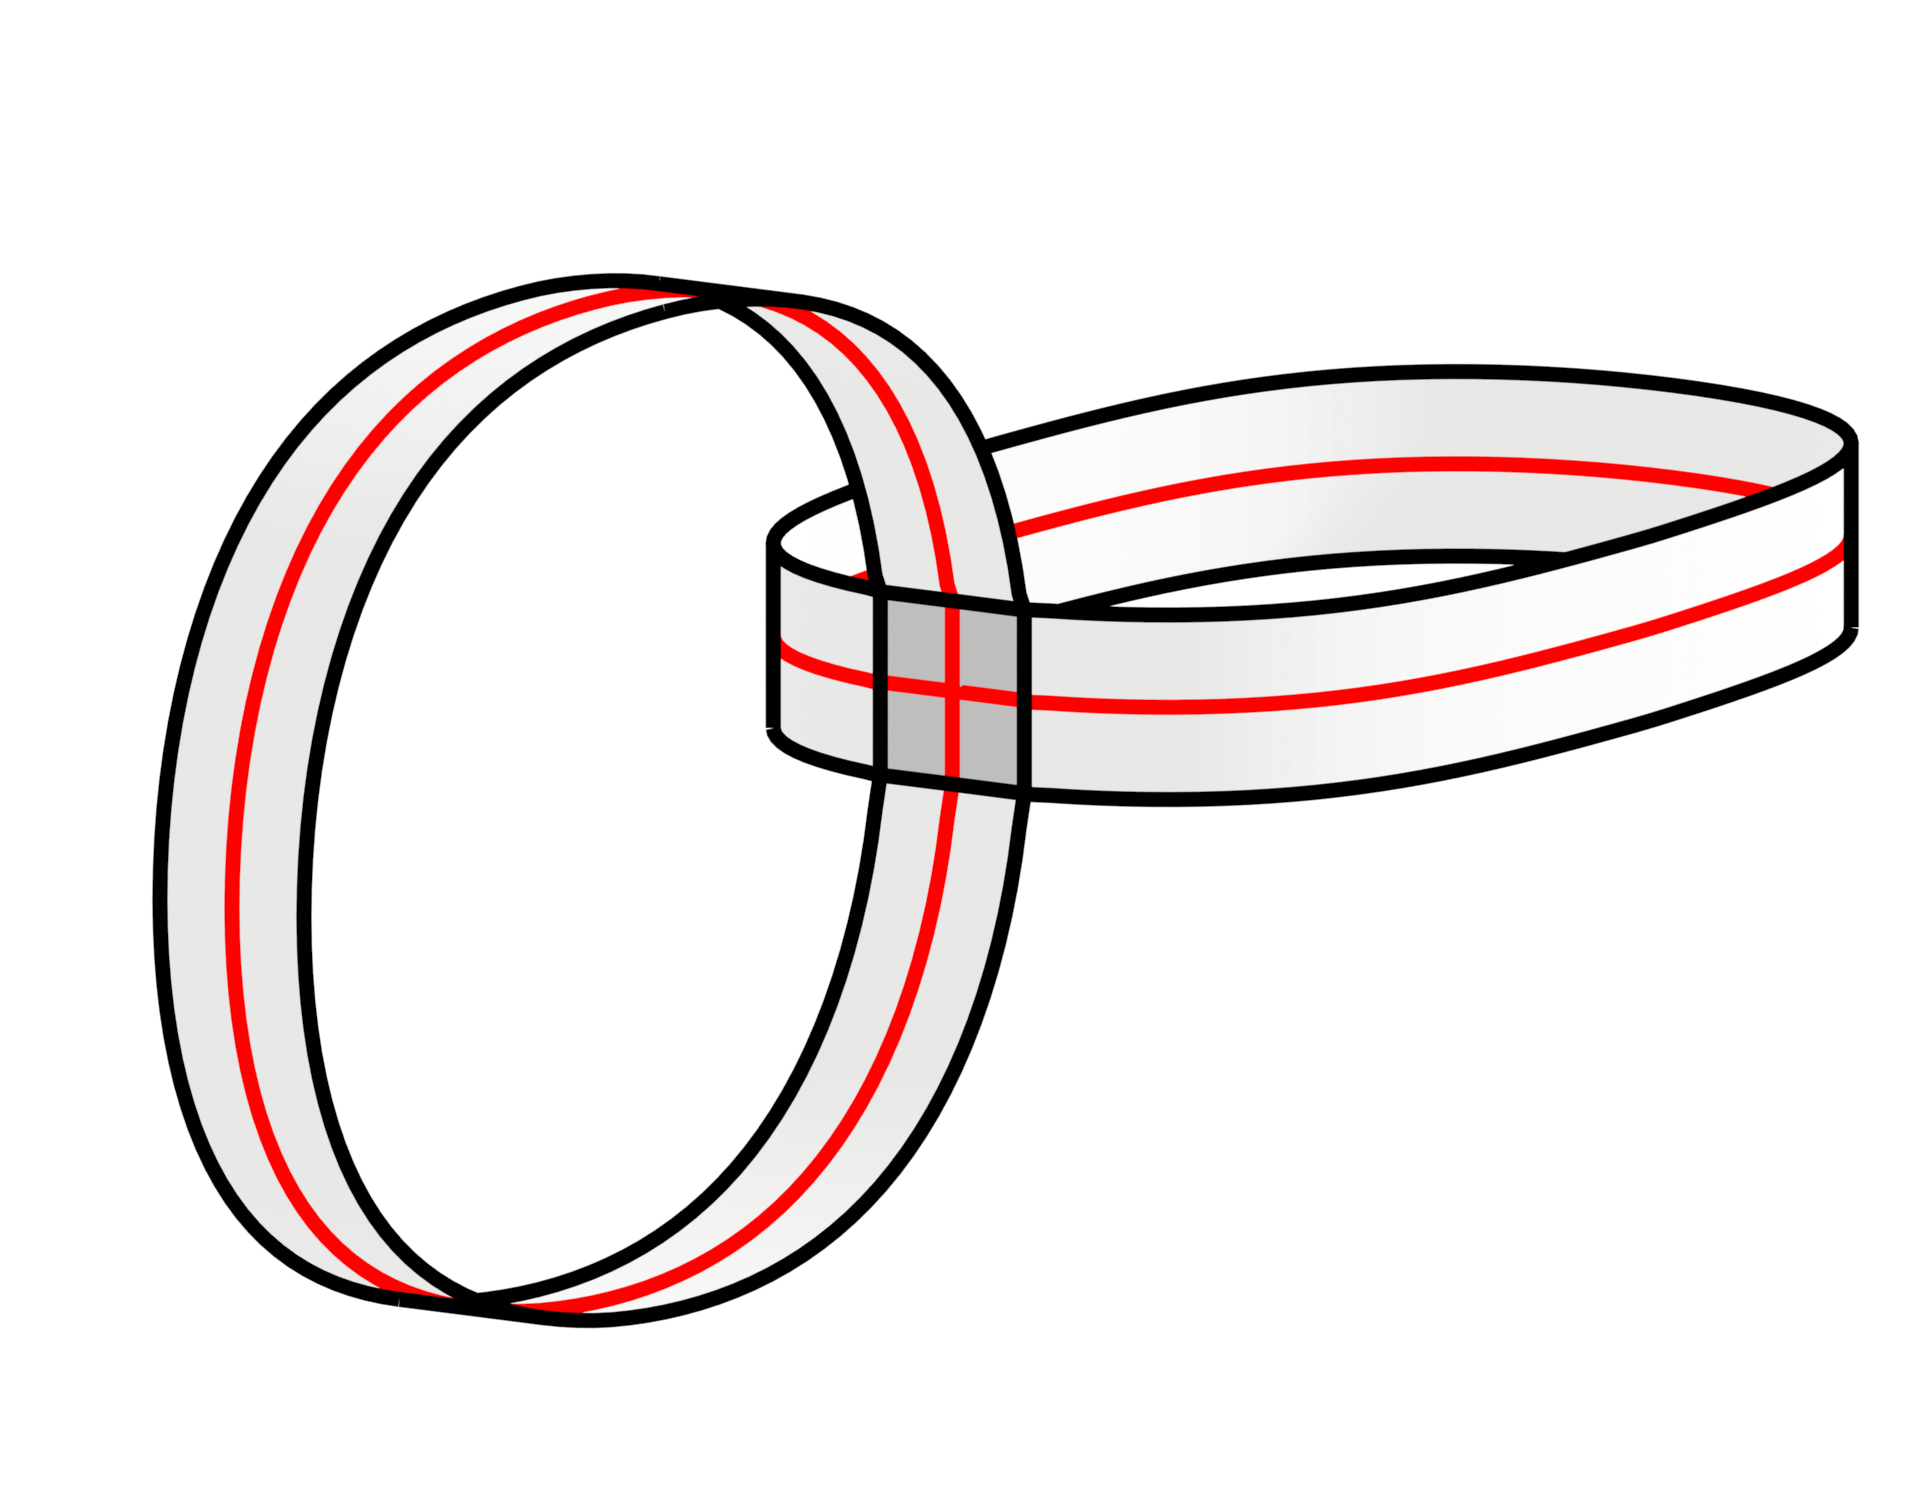
\includegraphics[width=3in]{graphics/temp-diagrams/disk-bundle-plumbing-example.png}
	\caption{Plumbing of two disk bundles.}\label{fig:disk-bundle-plumbing-example}
\end{figure}

\begin{theorem}
	Let $Q$ be a symmetric $n\times n$ integer matrix with even entries on the diagonal.There exists a highly-connected $4k$-manifold $P^{4k}(Q)$ with highly-connected boundary $\partial P^{4k}(Q)$ such that $Q$ is the matrix of the intersection form on $\H^{2k}(P^{4k}(Q), \partial P^{4k}(Q))$.
\end{theorem}

\pagebreak
\subsection*{Dodecahedral Space}

We know that there are no exotic spheres in dimension $3$, but what happens if we repeat the $\E_8$-plumbing construction in $4$-dimensions? While the boundary of the resulting manifold is not an exotic sphere, it has the homology of a $3$-sphere yet is not homeomorphic to the standard $3$-sphere.
This $3$-manifold is known as (Poincar\'e) \defn{dodecahedral space} and has a beautiful geometric construction. We'll denote this space by $\mathscr{D}$. Aside from being a wonderful example of a non-Euclidean geometry, this space also was the first counter-example to an incorrect earlier form of the Poincar\'e hypothesised which stated that every homology $3$-sphere was also homeomorphic to the $3$-sphere. Much like exotic spheres are counter-examples to the smooth Poincar\'e hypothesis, in a similar vein the dodecahedral space can be thought of as a sort of ``proto exotic sphere'' serving as a counter-example to the ``proto Poincar\'e hypothesis''.

The classic construction of dodecahedral space $\mathscr{D}$ is due to Poincar\'e \todo{cite}. We begin by letting $\mathcal{D}\subset \R^3$ be a solid dodecahedron in three dimensional Euclidean space. The dodecahedron has 6 pairs of opposite pentagonal faces. Picking a clockwise spherical orientation on $\mathcal{D}$, we can glue together opposing faces with a minimal clockwise twist to line them up (see \cref{fig:dodecahedral_space_construction}). The resulting quotient space is a closed $3$-manifold, and this manifold is dodecahedral space $\mathscr{D}$.

\begin{figure}[ht]
	\centering
	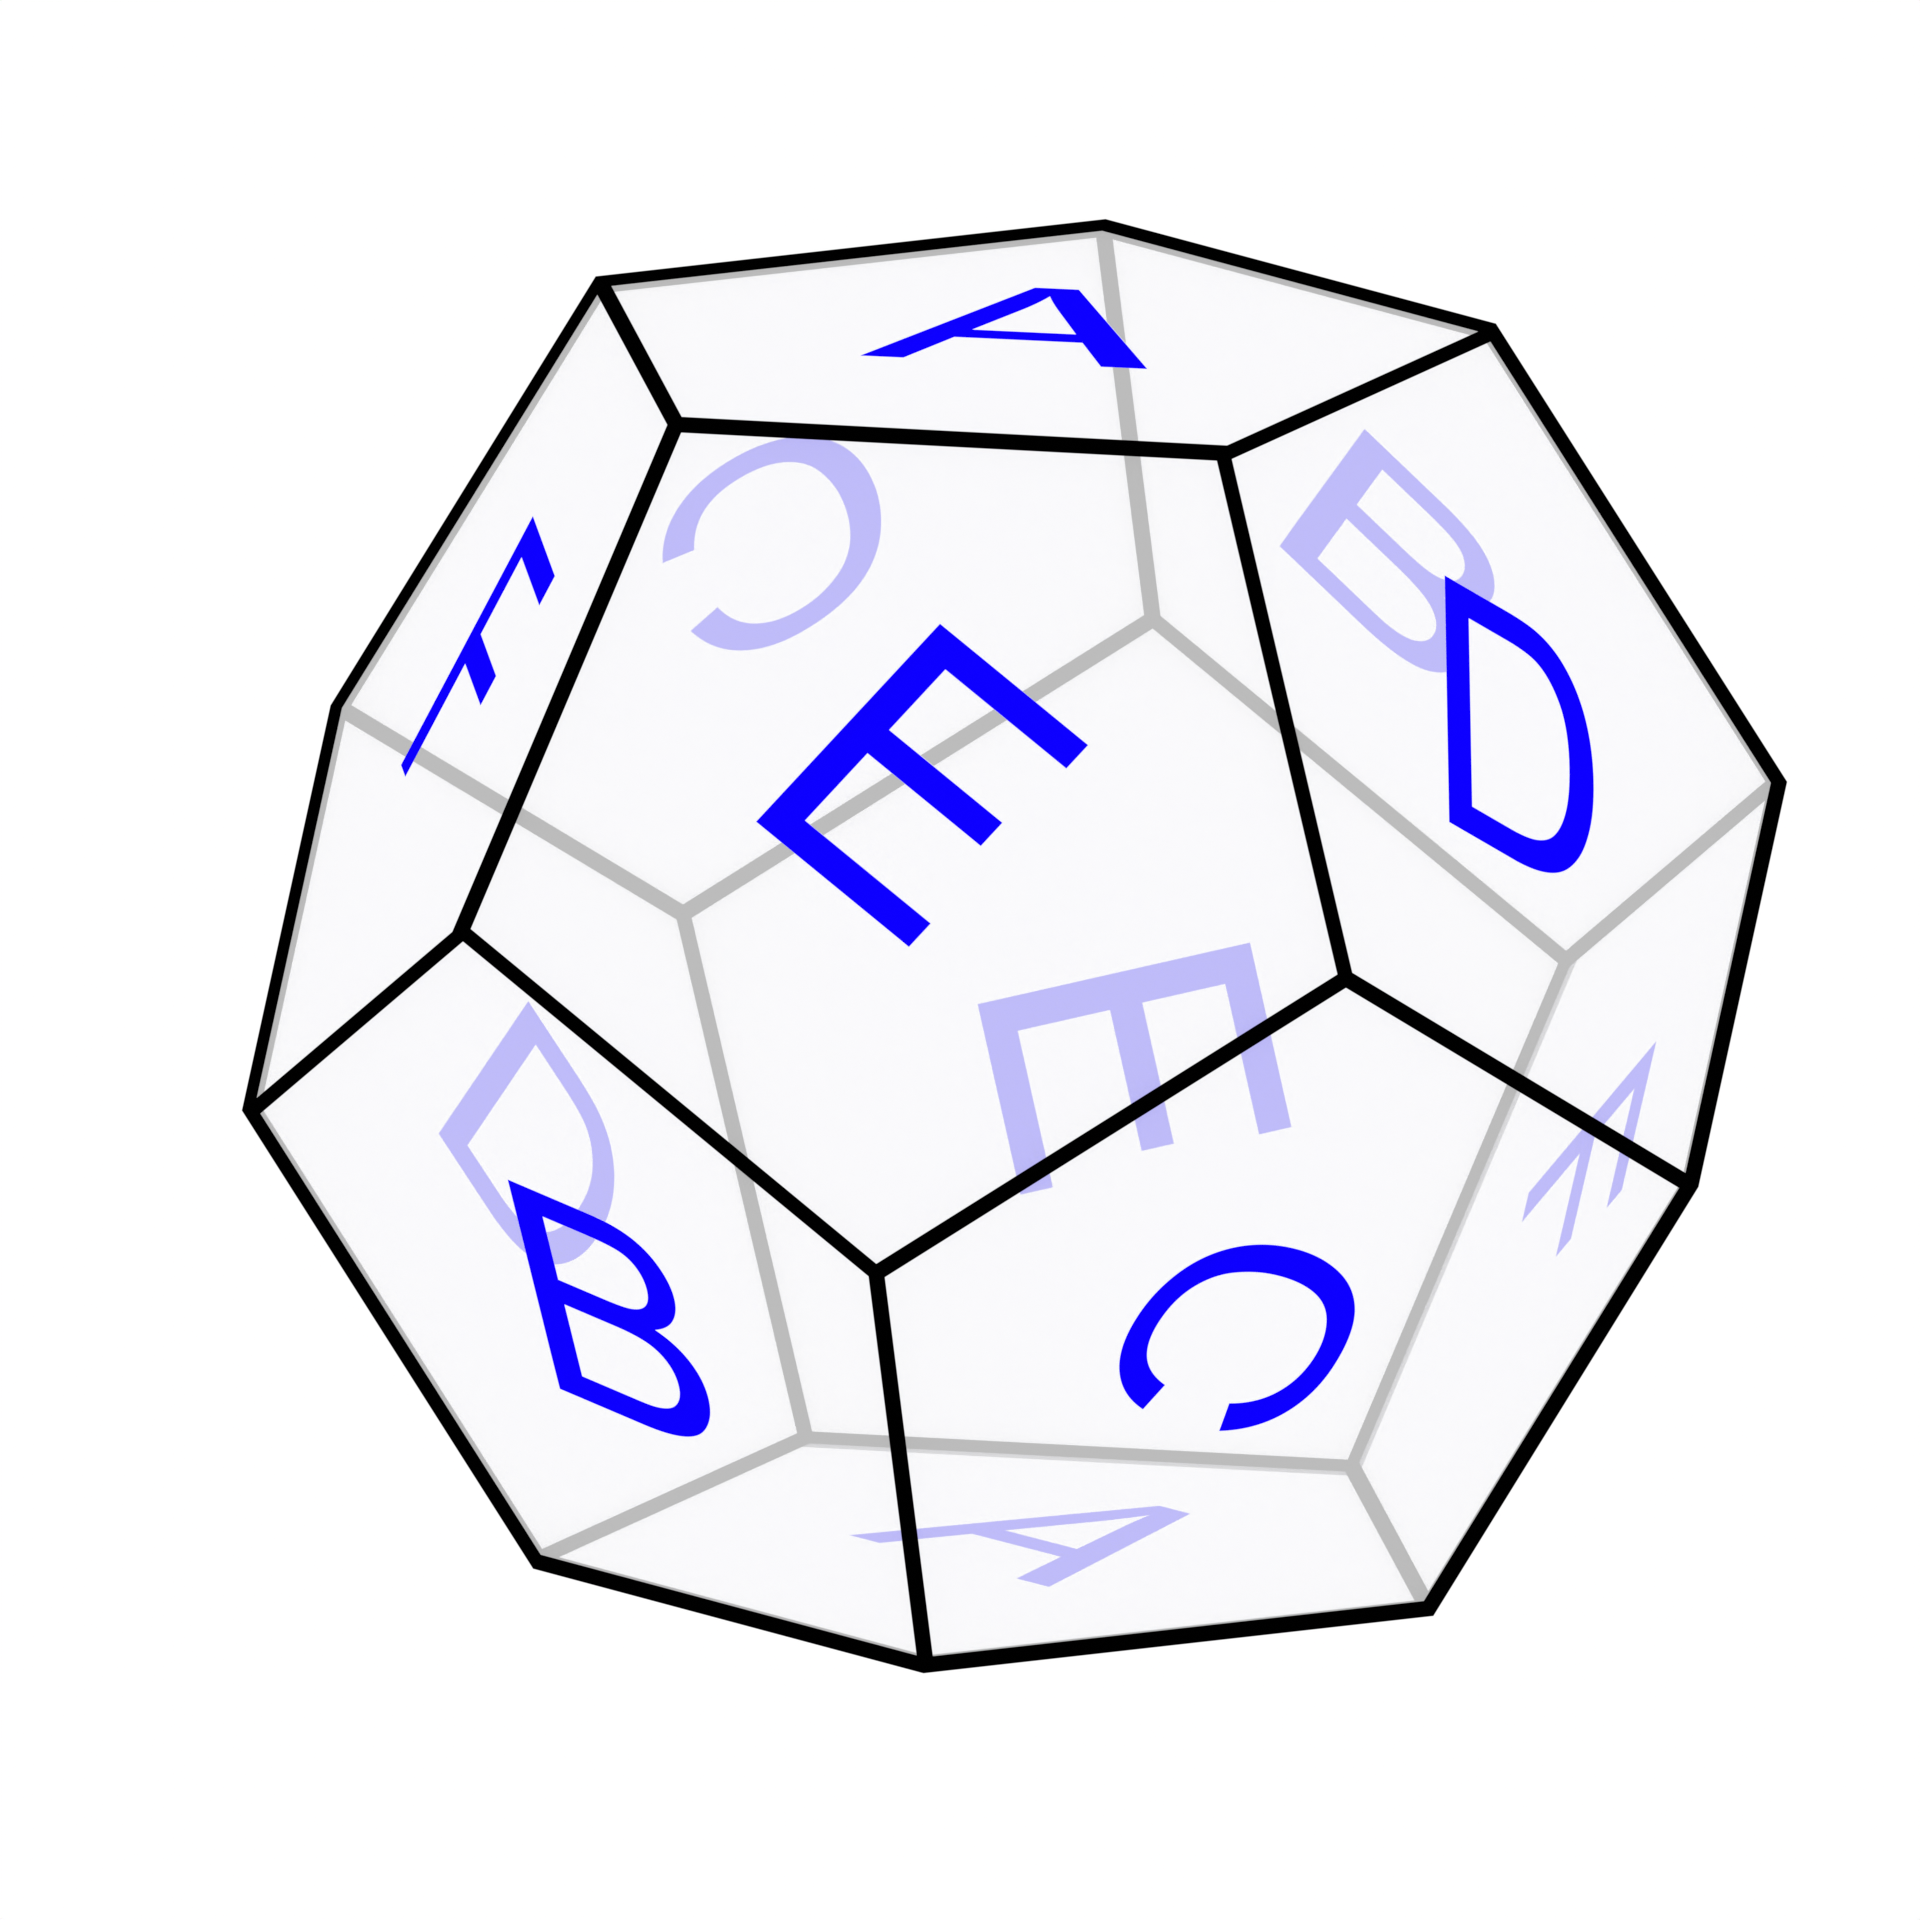
\includegraphics[width=2in]{graphics/temp-diagrams/dodecahedral-space-geometric-construction.png}
	\caption{Construction of Dodecahedral Space}\label{fig:dodecahedral_space_construction}
\end{figure}

Given this geometric construction, it should be fairly straightforward -- albeit tedious -- to compute the homology of dodecahedral space by means of a cellular decomposition. After such a computation, we would find that:
\begin{proposition}
	Dodecahedral space is a homology $3$-sphere.
\end{proposition}

While the first homology of dodecahedral space is trivial and incapable of differentiating dodecahedral space from a 3-sphere, the fundamental group reveals a much richer geometric structure. If we let $\SO_3$ act on $\R^3$ in the usual way, we can form the symmetry group $\Sym(\mathcal{D})\subset \SO_3$ of orientation preserving orthogonal transformations which leave the dodecahedron $\mathcal{D}$ unchanged. This is known as the \defn{icosahedral group}\footnote{The icosahedron and dodecahedron are dual, so the choice of icosahedral in the name is purely a historical convention.} $\mathrm{I}\subset \SO_3$, a group containing $60$ elements and isomorphic to the alternating group $A_5$. There is a double cover of $\SO_3$ by the $\Spin_3$ Lie group:
\[
	\SU_2\cong \Spin_3\lkxto[2:1] \SO_3
\]
The \defn{binary icosahedral group}, denoted $2\mathrm{I}$, is the preimage of $\mathrm{I}$ under this double cover and hence contains $120$ elements. Since there is an exceptional isomorphism $\SU_2\cong \Spin_3$, the binary icosahedral group admits a representation by unitary complex $2\times 2$ matrices.
We then have:
\begin{proposition}
	The fundamental group of dodecahedral space is the binary icosahedral group.
\end{proposition}
This hints at another interesting fact about the binary icosahedral group -- it is a \defn{perfect group}, which means that it's commutator subgroup is the entire group. By the Hurewicz isomorphism, it would follow that
\[
	\H_1(\mathscr{D}) \cong \Ab\left[ \pi_1(\mathscr{D})\right] \cong 2\mathrm{I}/[2\mathrm{I}, 2\mathrm{I}] = 0
\]
where $\Ab$ denotes the abelianization. This perfectness of the fundamental group thus ``hides'' the non-trivial topology of $\mathscr{D}$ from being detectable by homology. It's interesting to note that dodecahedral space and $S^3$ are the only homology $3$-spheres up to homeomorphism with finite fundamental groups.

There is also a useful construction of dodecahedral space which will later appear in our later study of Brieskorn manifolds in \cref{sec:brieskorn-manifolds}. If we identify $\SU_2$ with the $3$-sphere of unit quaternions, we obtain the construction:

\begin{proposition}
	There is a diffeomorphism $\mathscr{D} \cong S^3 / 2\mathrm{I}$ expressing dodecahedral space as the quotient of the $3$-sphere under a proper group action by $2\mathrm{I}$.
\end{proposition}

Finally, let's see how the dodecahedral space and binary icosahedral group arises out of the plumbing construction we've worked with thus far.

\todo{write this section}

\begin{proposition}
	There is a diffeomorphism $\mathscr{D}\cong \partial P^4(\E_8)$.
\end{proposition}

	\todo{citations}

\begin{remark}
  In the early 2000's, the Wilkinson Microwave Anisotropy Probe (WMAP) was launched to accurately map out the cosmic microwave background, i.e. leftover heat from the Big Bang. The observed lack of temperature correlations above 60$^\circ$ led astrophysicist Jean-Paul Luminet to propose a cosmological model \cite{luminet2003dodecahedral} where the shape of the universe is a dodecahedral space, explaining the lack of large scale correlations by means of the compact topology of space. In such a finite universe, larger temperature correlations simply wouldn't have enough room to form.
  While this model made some predictions aligning with observed cosmological data
  \cite{roukema2008dodecahedral}, higher resolution data by the later Planck spacecraft later seemed to suggest that the observable large scale topology is trivial, leading to the modern prevalence of the $\Lambda$CDM model as a standard model for cosmology.
\end{remark}
